%!TEX root = ../main.tex

\section{Evaluation}
%In this section, w
We have implemented our hybrid rule learning approach within a %the
system prototype RuLES in \ds{software details, e.g., language, etc }%of 
and conducted experiments on a machine with 80 cores and 500GB RAM\ds{are these details of the machine correct?}.
In this section we report %and conducted 
the results of our experimental evaluation, which focuses on 1) the benefits of our hybrid embedding-based quality measure over traditional rule measures; 2) the effectiveness of RuLES against the state-of-art Horn rule learning system; (3) the quality of nonmonotonic rules learned by RuLES compared to the existing methods.
%The purpose of the experimental evaluation is to evaluate 
%First, we evaluate .
%Second, we %test the effectiveness of 
%approaches, 
%Finally, we test the quality of nonmontonic rules learned by RuLES against the existing methods. 
%nonmontonic rule revision systems.
% , the .

\subsection{Experimental Setup}
\leanparagraph{Data sets}
All experiments were performed on %In 
the following %experiments we used 
2 real world data sets: 
\squishlist
\item \textit{FB15K}~\cite{Bordes:NIPS2013}: a subset of Freebase with 592K binary facts over 15K entities and 1245 relations %, this KG is 
commonly used for evaluating KG embedding models~\cite{DBLP:journals/tkde/WangMWG17}.
\item \textit{WIKI44K}: a subset of %subset of 
Wikidata dataset from December 2014 with 250K binary facts over 44K entities and 100 relations %creating  %used by AMIE
used in~\cite{amie}.
%. The subset contained . The restriction is imposed to allow the construction of embedding models within reasonable computational  resources.

\item \textit{Family}~\cite{NeuralLP}: a knowledge graph containing 28K binary facts over 3K entities and 12 relations. \thi{this added for NeuralLP}
\squishend

Since obtaining a real life complete ideal KG $\cG^i$ is hard, we used the existing %data set 
KG as a reference graph $\cG^i_{appr}$ approximating $\cG^i$. For each KG, we randomly selected $80\%$ of facts while preserving the distribution of facts over predicates 
%\ds{for every relation?}
 as the available graph, which we refer to as $\cG^a$.
%, while the remaining represent the missing facts to-be-predict during experiments.%\gad{any other usage?}

\leanparagraph{Embedding models}
We experimented with the three state-of-the-art embedding models: %, namely, 
TransE \cite{Bordes:NIPS2013}, HolE \cite{DBLP:conf/aaai/NickelRP16}, and the text-enhanced SSP \cite{DBLP:conf/aaai/0005HMZ17} model. 
%We trained them on the available graph, which we refer to as $\cG^a$. %However, f
%For 
%To train 
TransE and HolE were trained on $\cG^a$ and SSP on $\cG^a$ enriched with %apart from the KG, we also %augmented %our graphs 
%$\cG^a$ with 
%
a textual description for each entity extracted from Wikidata %\ds{for every entity?}. 
%Since the performance of each model varies %according to 
%depending on the %the 
%dataset; 
We compared the %used the remaining facts in $\cG^i_{appr}$ to compute %about 
effectiveness of the models and selected for every KG %among 
the best one. Apart from SSP, which showed the best performance on both KGs we also selected %i.e., 
HolE for \textit{FB15K} and TransE for \textit{Wiki44K}. %The text-enhanced model SSP showed the best performance and thus was also chosen. %model. % on the data sets. 
%Accordingly, we used HolE %to encode 
%For \textit{FB15K} %(\ie performs better than TransE), %while we utilized 
% Furthermore, we %also 
%compared to SSP as \textit{text enhanced} model, which independently performs better than both TransE and HolE on both datasets. It is worth noting that 
Note that in this work as a proof of concept we considered some of the most popular embedding models, but %while we utilized some of the most popular %se models as a proof of concept, 
conceptually any model (see \cite{DBLP:journals/tkde/WangMWG17} for overview) can be plugged in in our system. %, yet other models can be adopted.


\leanparagraph{Evaluation metric} 
In these experiments, we use the quality of predictions produced %through applying the 
by the learned rules on $\cG^a$ as the evaluation criteria, i.e., the more correct facts %predictions 
beyond %the actual graph 
$\cG^a$ a ruleset produces, the better it is. %the rule set. 
%Therefore, if the result of applying rule $r$ on $\cG^a$ is $\cG^a_r$ we only consider the new predictions  $\cG^a_r \setminus \cG_a $, \ie do not already exist in $\cG^a$.
We consider two evaluation settings: closed world setting and open world setting. In the former, the quality of a rule $r$ is estimated by the ratio of predictions in $\cG^i_{\mi{appr}}$ to the number of all predictions in $\cG^a_r\backslash \cG^a$, i.e., 
% First, we define the prediction precision for a rule in the closed world as the ratio of the correct new predictions exist in $\cG^i_{appr}$ to the total number of new prediction:    
 \[   pred\_prec_{CW}(r) = \frac{|\cG^a_r \cap \cG^i_{appr} \setminus \cG^a|}{|\cG^a_r \setminus \cG_a|}\]
and for a rule set $R$, we define \textit{prediction precision} as
 \[   pred\_prec_{CW}(R) = \frac{\sum\limits_{r\in R} pred\_prec_{CW}(r)}{|R|}.\]
%, we define the \textit{prediction precision} as the average of $pred\_prec_{CW}(r)$ for all $r \in R$.% as an aggregated \textit{prediction precision}.
In the open world setting, we also account for the quality of predictions outside $\cG^i_{\mi{appr}}$ by performing a random sampling and manually annotating the sampled facts relying on Web resources such as Wikipedia. %Furthermore, in order to include the predictions outside the $\cG^i_{appr}$ in the evaluation, a sample of predictions is randomly picked and manually annotated based on web resources such as Wikipedia. 
We define the OW prediction precision $\mi{pred\_prec_{OW}}$ for a set of rules $R$ as follows:
\[pred\_prec_{OW}(R) = \frac{|\cG'\cap \cG^i_{\mi{appr}}|+|\cG'\backslash \cG^i_{\mi{appr}}|\times \mi{accuracy(\cG'\backslash \cG^i_{\mi{appr}})}|}{|\cG'|}\]
%|\cG'\backslash \cG^i_{\mi{appr}}\times \mi{accuracy(\cG'\backslash \cG^i_{\mi{appr}})}|}{|\cG'\backslashcG^a|},\]
where $\cG'=\bigcup_{r\in R}\cG^a_r\backslash \cG^a$ is the union of predictions generated by rules in $R$, and $\mi{accuracy(S)}$ is the approximated ratio of true facts inside $S$ computed via manual checking of facts sampled from $S$.
%\gad{missing How do we combine? }
\ds{fixed, please add intuitive explanations}. %the closed world \textit{prediction precision} to compute the open world prediction precision $pred\_prec_{OW}$ the as: $pred\_prec_{OW}$
Finally, to evaluate the meaningfulness of %chosen negated atoms 
exceptions in a rule (i.e., negated atoms) we compute %by computing 
the \textit{revision precision}, which according to~\cite{trantowards} is defined as the ratio of incorrect %new 
facts in the difference between predictions produced by the Horn part of a rule and its nonmonotonic version over %that were removed by adding the negated %part
%atoms to 
the total number of predictions in this difference (the higher the revision precision, the better the rule exceptions) computed per ruleset. Formally,
\[rev\_prec_{OW}(R) = 1-\frac{|\cG'' \cap \cG^i_{\mi{appr}}|+|\cG''\backslash \cG^i_{\mi{appr}}|\times \mi{accuracy(\cG''\backslash \cG^i_{\mi{appr}})}|}{|\cG''|}\]\\
where $\cG''=\cG_H\backslash \cG_R$, where $H$ is the set of Horn parts of rules in $R$. 
Intuitively, $\G''$ contains predictions not produced by the rules in $R$ but by their Horn version. 

%\ds{is it computed per rule or ruleset? should we add a formula like for the prediction score?}. \gad{it is computed per set of rules no need for extra info} %removed facts, . %. The lower the \textit{revision score}, the better the nonmontonic rules.
 
 
% \leanparagraph{RuLES configuration} % Beside the KG, RuLES expects a precomputed embedding model, language constrains as an input, and the minimum support of the rules body, the minimum head coverage, the minimum embedding based confidence, and the embedding weight value. 
%We run RuLES in several configurations:
%\textit{RuLES-T}, \textit{RuLES-H}, and \textit{RuLES-S} with $\mu_2$ computed relying on TransE, HolE, and SSP models respectively. For each configuration we also distinguish $\mu_1$ used: 
%%Each instance uses either 
%either \textit{standard confidence} or \textit{PCA confidence} (marked with suffix \textit{-Conf} \textit{-PCA} respectively).
%The rest of the parameters used by RuLES were set as follows: \gad{do we have any other of these parameters fixed in all experiments?}\ds{TODO: if so, please add $\mi{min\_hc=}$, $\mi{min\_conf}$, $\mi{min\_}....$}

\leanparagraph{RuLES configuration} 
We run RuLES in several configurations where $\mu_1$ is set to either \textit{standard confidence} (Conf) or \textit{PCA confidence} (PCA), and $\mu_2$ is computed based on either TransE, HolE, or SSP models %(abbreviated as \textit{T}, \textit{H}, and \textit{S}). 
Though the experiments configurations are named as \textbf{$\mu_1$-$\mu_2$} (\eg Conf-HolE).
The rest of the parameters used by RuLES were set as follows: \gad{do we have any other of these parameters fixed in all experiments?}\ds{TODO: if so, please add $\mi{min\_hc=}$, $\mi{min\_conf}$, $\mi{min\_}$..}



%\leanparagraph{Baselines} We compare RuLES to:
%\gad{not sure if we should leave these to the corresponding experiments}
%\ds{better to shift these to the respective experiments (left here for now)}
%\squishlist
%\item \textit{AMIE-PCA}~\cite{amie}: is a state-of-art Horn rule learning system. In this variant, we are using the system with their PCA confidence metric. AMIE requires as an input a KG, minimum support, head coverage and confidence values, and maximum rule length.
%\item \textit{AMIE-Conf}: where we configured AMIE to use the standard confidence measurement instead of the PCA confidence.
%\item \textit{RUMIS}~\cite{trantowards}: Nonmonotonic rule revision system. It takes a set of horn rules and revise them by adding negating atoms representing the expectations in the KG. 
%\squishend




\subsection{Embedding-based hybrid quality function}

\captionsetup[subfigure]{textfont=scriptsize}
 \begin{figure}[t]
     \centering
      %Gad: to unify legend and save space
     \subfloat{{
\includegraphics[width=0.6\textwidth]{figures/new_exp1/legend-crop.pdf} }}\\[-1ex]
     \setcounter{subfigure}{0}
     \subfloat[Conf-HolE on FB15K]{{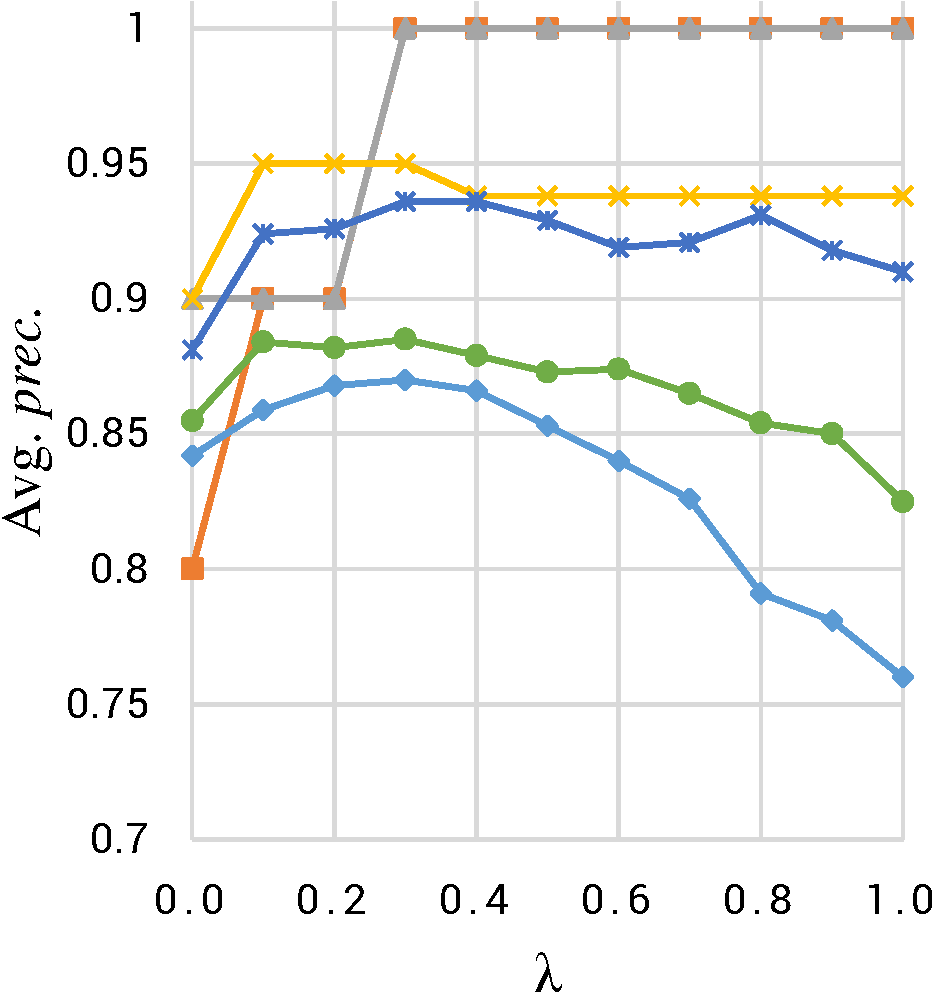
\includegraphics[width=0.3\textwidth]{figures/new_exp1/fb15k_hole_conf-crop.pdf} }\label{fig:fb-HoLE-Conf}}
     \subfloat[Conf-SSP on FB15K]{{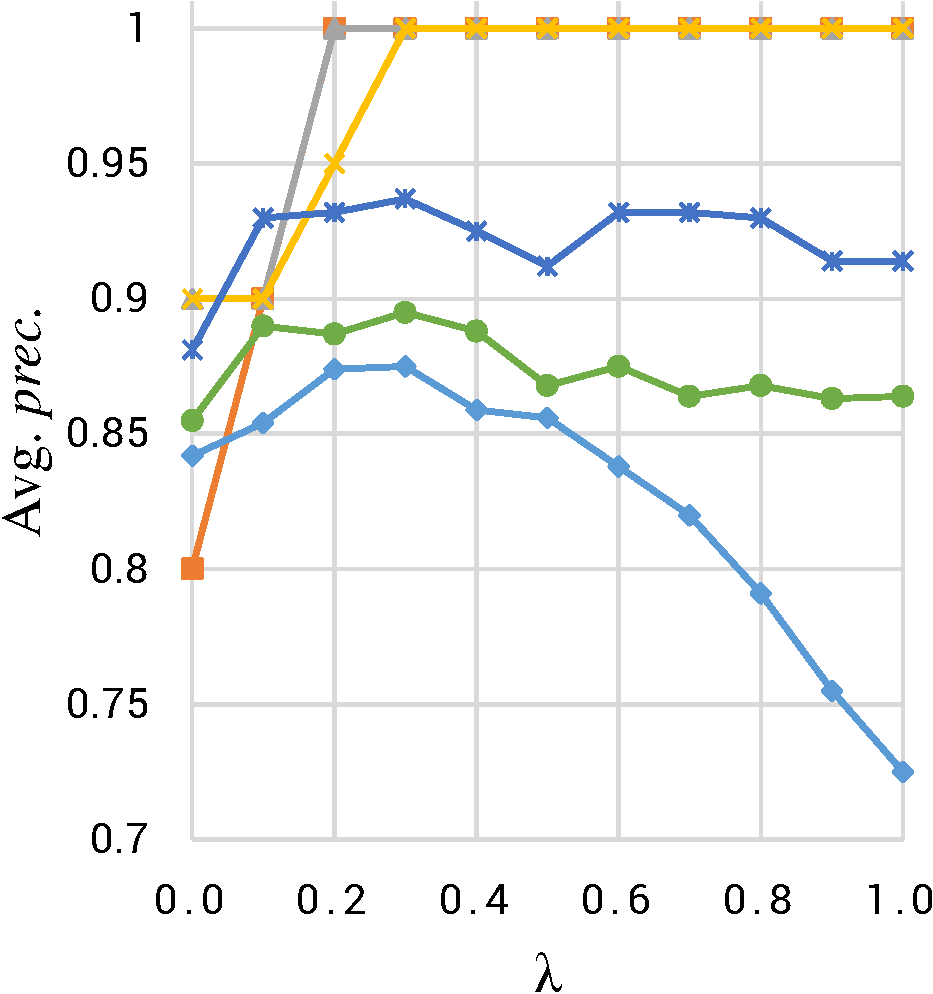
\includegraphics[width=0.3\textwidth]{figures/new_exp1/fb15k_ssp_conf-crop.pdf} \label{fig:fb-SSP-Conf}}}
     %\subfloat[RulES-H-PCA on FB15K]{{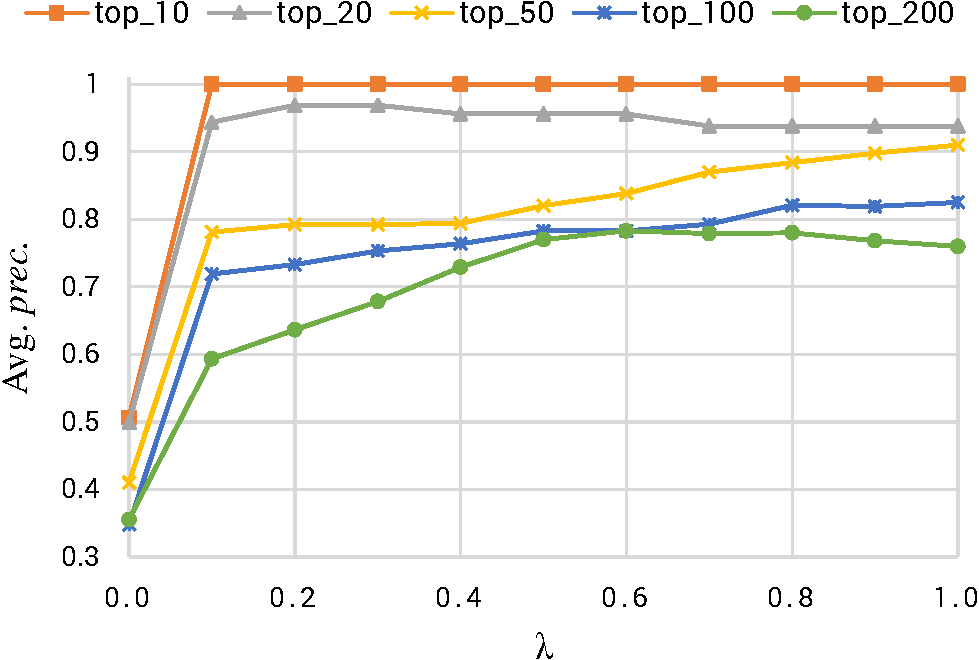
\includegraphics[width=0.3\textwidth]{figures/fb15k_hole_pca-crop.pdf} }}
    \subfloat[PCA-SSP on FB15K]{{\includegraphics[width=0.3\textwidth]{figures/new_exp1/fb15k_ssp_pca-crop.pdf} }\label{fig:fb-SSP-PCA}} \\   
    
    \subfloat[Conf-TransE on Wiki44K]{{\includegraphics[width=0.3\textwidth]{figures/new_exp1/wiki44k_transe_conf-crop.pdf} }\label{fig:wi-TransE-Conf}}
    \subfloat[Conf-SSP on Wiki44K]{{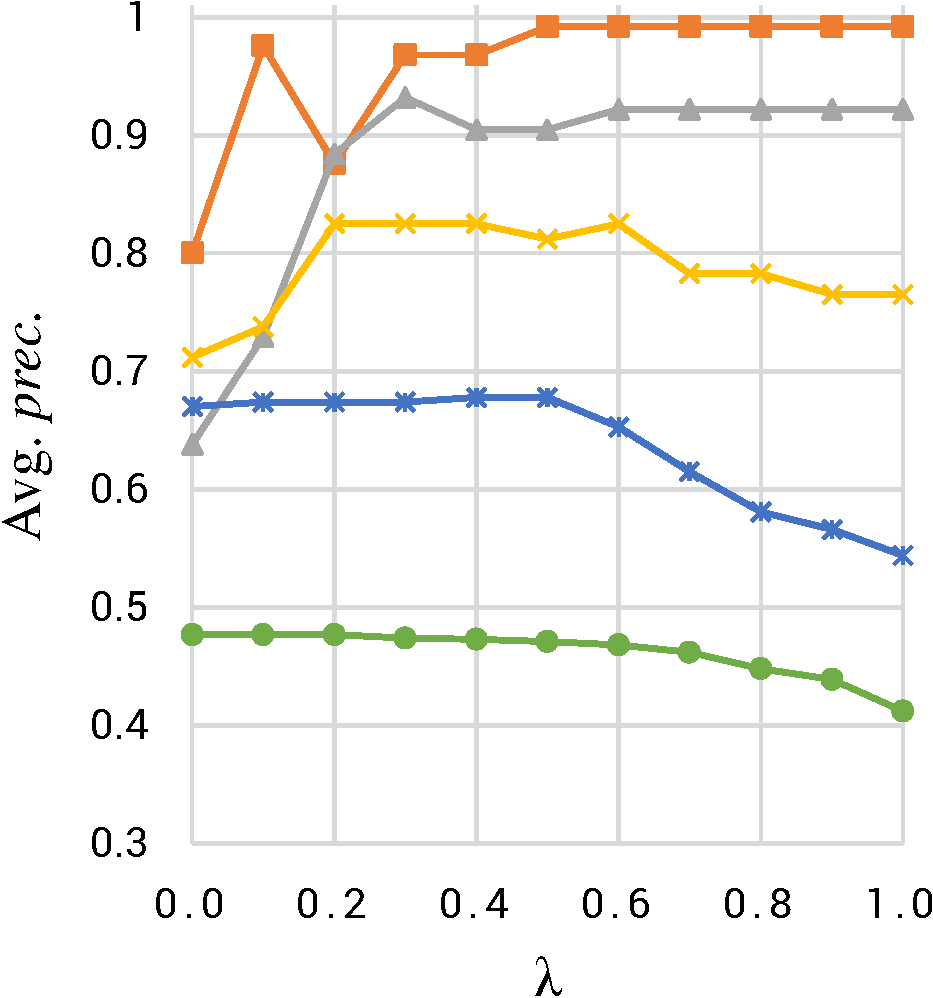
\includegraphics[width=0.3\textwidth]{figures/new_exp1/wiki44k_ssp_conf-crop.pdf} }\label{fig:wi-SSP-Conf}}
     %\subfloat[RulES-H-PCA on Wiki44K]{{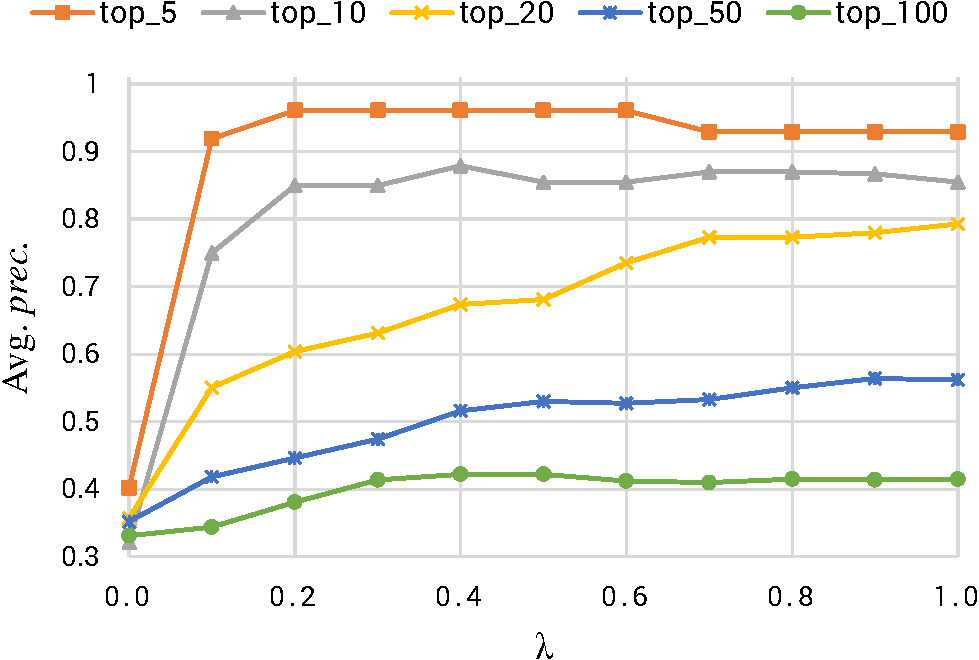
\includegraphics[width=0.3\textwidth]{figures/wiki44k_transe_pca-crop.pdf} }}
     \subfloat[PCA-SSP on Wiki44K]{{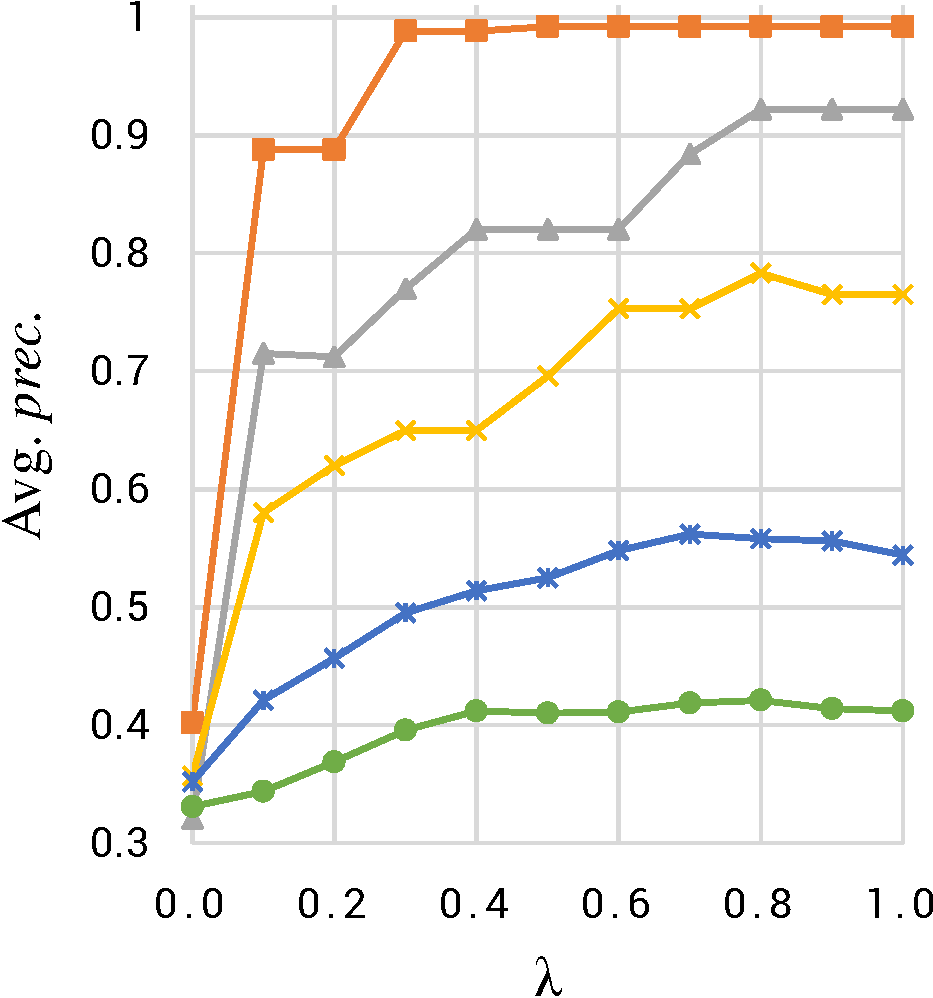
\includegraphics[width=0.3\textwidth]{figures/new_exp1/wiki44k_ssp_pca-crop.pdf} }\label{fig:wi-SSP-PCA}} \\  
    
     \caption{$pred\_prec_{CW}$ of the \textit{top-k} rules with various \textit{embedding weights}.}
     \label{fig:diff_lambda}
 \end{figure}
%\captionsetup[subfigure]{labelformat=empty}
%\begin{figure}[t]
%    \centering    
%    % \vspace*{-3mm}
%    \subfloat{{
\includegraphics[width=0.5\textwidth]{figures/new_exp1/legend-crop.pdf} }}\\[-2ex]
%    \subfloat[FB15K(conf + HolE)]{{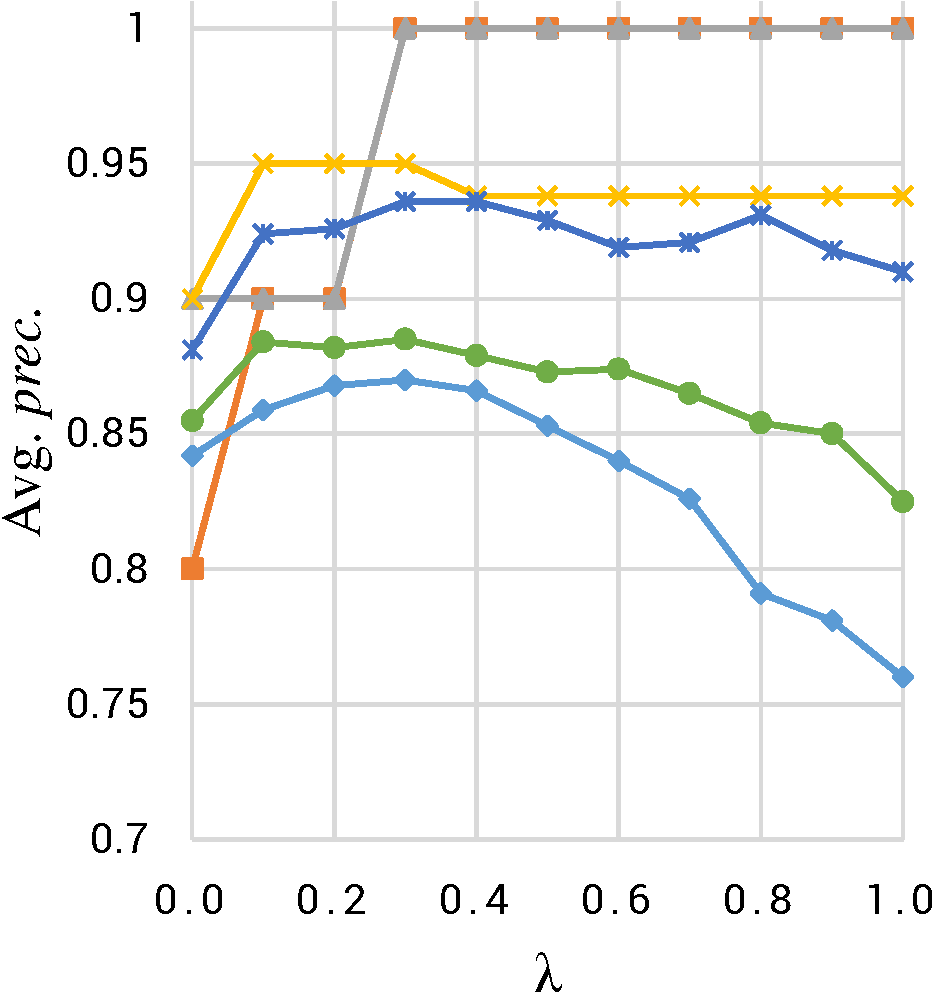
\includegraphics[width=0.33\textwidth]{figures/new_exp1/fb15k_hole_conf-crop.pdf} }}
%    \subfloat[FB15K(conf + SSP)]{{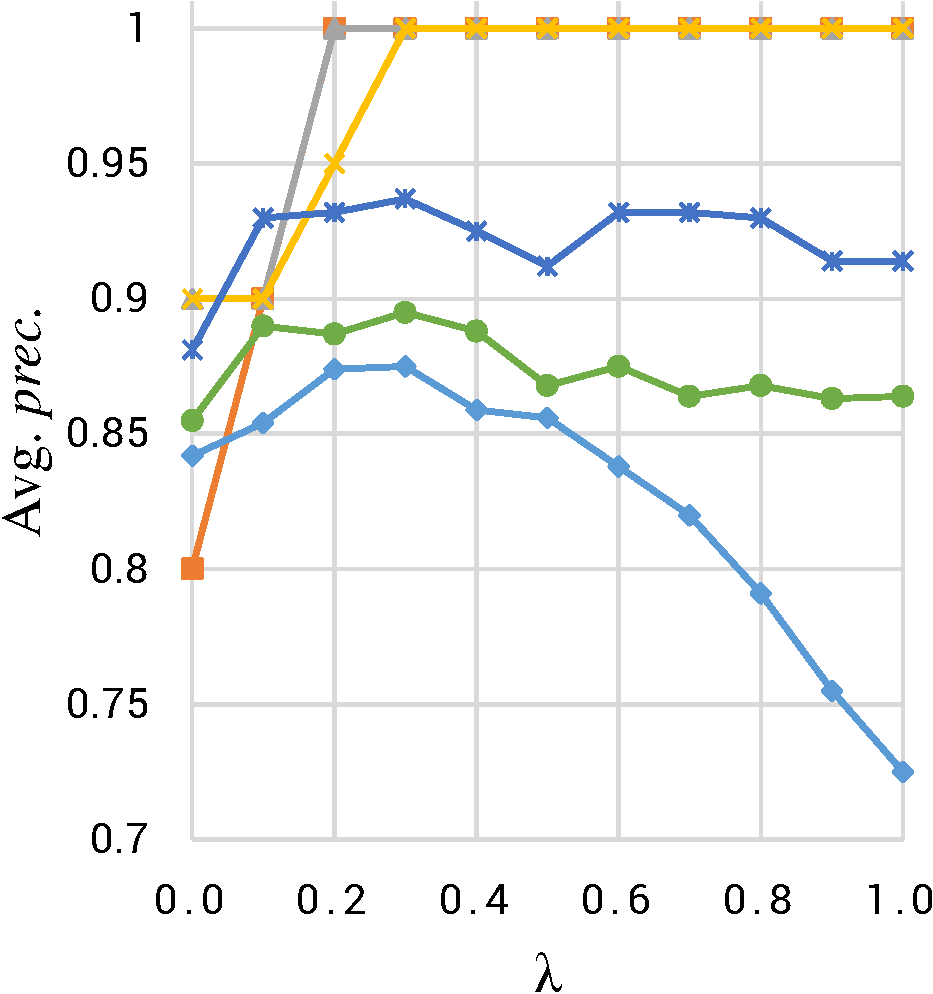
\includegraphics[width=0.33\textwidth]{figures/new_exp1/fb15k_ssp_conf-crop.pdf} }}
%    % \subfloat[PCA Confidence + HolE]{{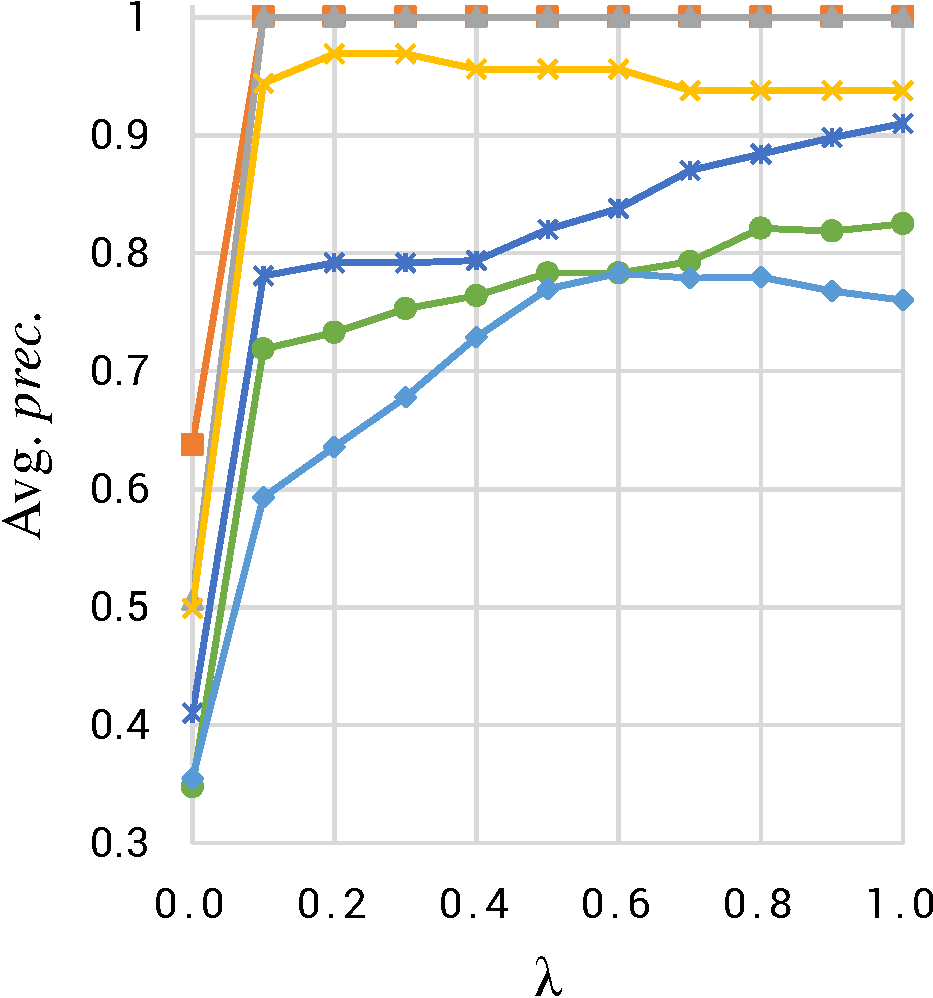
\includegraphics[width=0.5\textwidth]{figures/new_exp1/fb15k_hole_pca-crop.pdf} }}
%    \subfloat[FB15K(pcaconf + SSP)]{{\includegraphics[width=0.33\textwidth]{figures/new_exp1/fb15k_ssp_pca-crop.pdf} }}\\
%    \subfloat[Wiki44K(conf + TransE)]{{\includegraphics[width=0.33\textwidth]{figures/new_exp1/wiki44k_transe_conf-crop.pdf} }}
%    \subfloat[Wiki44K(conf + SSP)]{{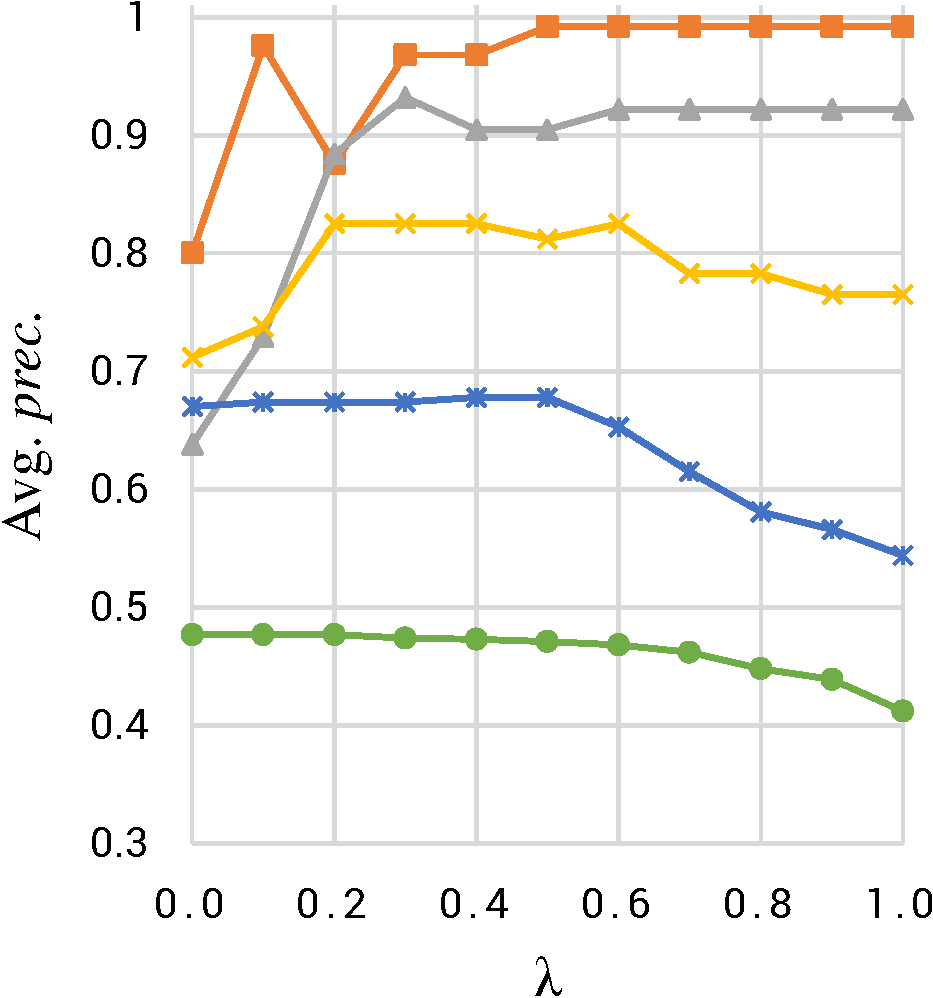
\includegraphics[width=0.33\textwidth]{figures/new_exp1/wiki44k_ssp_conf-crop.pdf} }}
%    % \subfloat[PCA Confidence + TransE]{{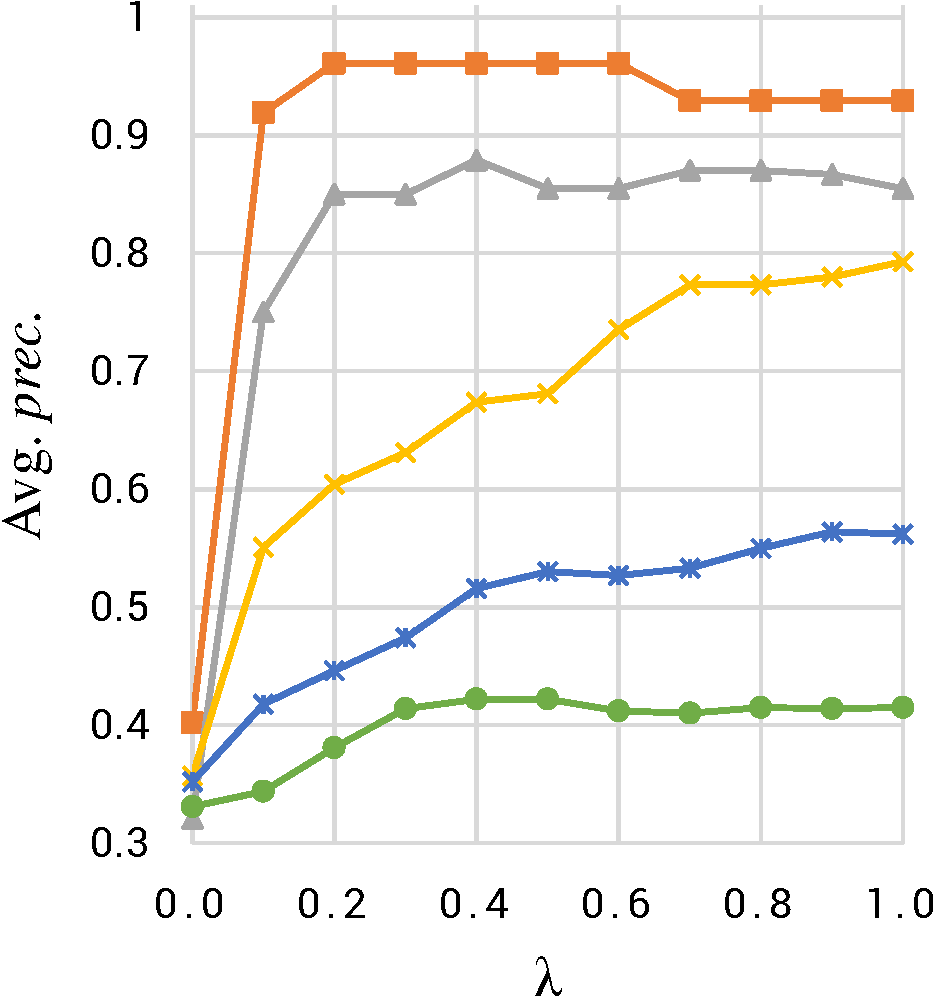
\includegraphics[width=0.5\textwidth]{figures/new_exp1/wiki44k_transe_pca-crop.pdf} }}
%    \subfloat[Wiki44K(pcaconf + SSP)]{{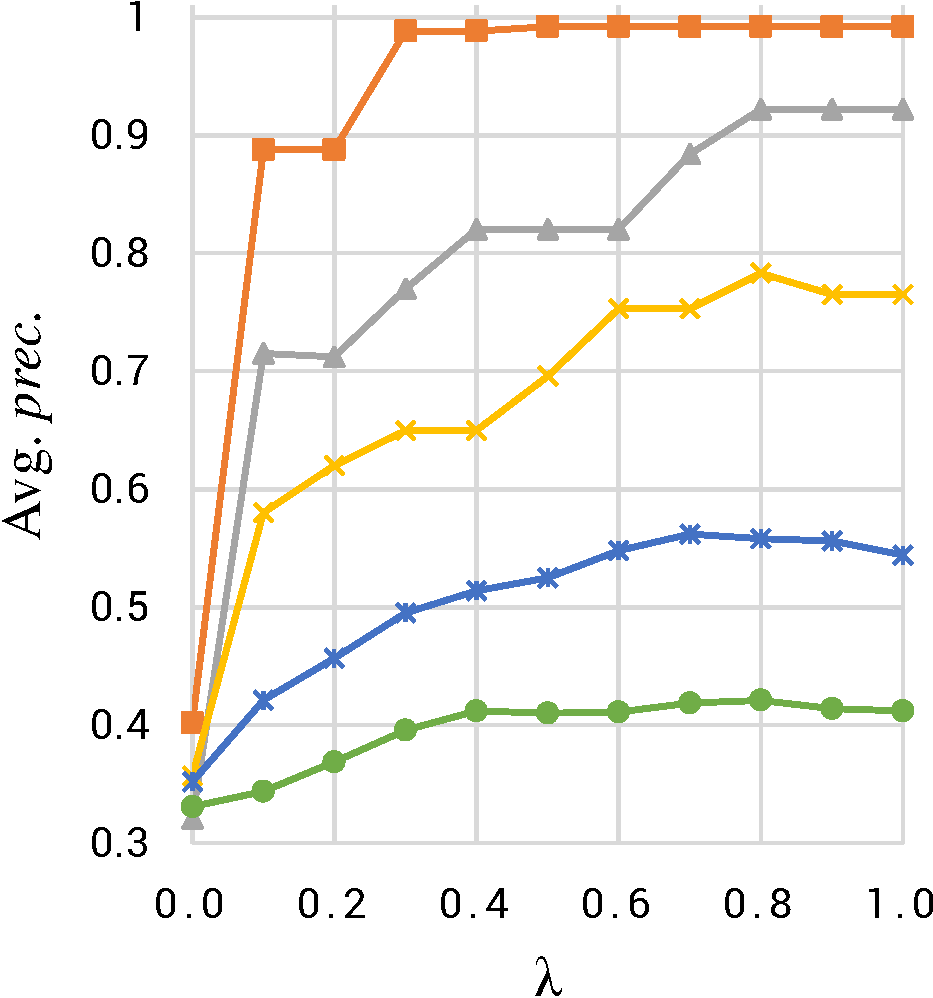
\includegraphics[width=0.33\textwidth]{figures/new_exp1/wiki44k_ssp_pca-crop.pdf} }}\\
%    
%    \caption{Avg. \textit{predictions precision} of the top rules with various \textit{embedding weights} \gad{figures labels should be updated and height should be reduced }}
%    \label{fig:fb15k_and_wiki44k}
%\end{figure}

\begin{table}[t]
\scriptsize
%\tiny
\centering
\begin{tabular}{c |r r r r |r r r r} 
 \multirow{3}{*}{\textbf{\textit{top-k}}} & \multicolumn{4}{c}{\textbf{FB15K}} & \multicolumn{4}{|c}{\textbf{Wiki44K}} \\
 \cmidrule{2-9}
 & \textbf{{~~}Conf}&  \textbf{{~~~~~~~~}PCA} & \textbf{Conf-HolE}& \textbf{Conf-SSP} &  \textbf{{~~}Conf}&  \textbf{{~~~~~~~~}PCA} & \textbf{Conf-TransE}& \textbf{Conf-SSP}\\
  & {\scriptsize($\lambda=0$)}  & {\scriptsize($\lambda=0$)} & {\scriptsize($\lambda=0.3$)} & {\scriptsize($\lambda=0.3$)} & {\scriptsize($\lambda=0$)} & {\scriptsize($\lambda=0$)} &{\scriptsize($\lambda=0.3$)} & {\scriptsize($\lambda=0.3$)}\\
 \midrule
 \textbf{5} & 0.800 & 0.638 & \textbf{1.000} & \textbf{1.000} & 0.800 & 0.402 & \textbf{0.995} & 0.968\\
\textbf{10} & 0.900 & 0.506 & \textbf{1.000} & \textbf{1.000} & 0.638 & 0.321 & 0.863 & \textbf{0.932} \\
\textbf{20} & 0.900 & 0.499 & 0.950 & \textbf{1.000} & 0.712 & 0.357 & 0.802 & \textbf{0.825}\\
\textbf{50} & 0.881 & 0.410 & 0.936 & \textbf{0.937} & 0.670 & 0.352 & \textbf{0.675} & 0.674 \\
\textbf{100} & 0.855 & 0.348 & 0.885 & \textbf{0.895} & \textbf{0.477} & 0.331 & 0.474 & 0.474\\
\textbf{200} & 0.842 & 0.355 & 0.870 & \textbf{0.875} & -- & -- & -- & -- \\
 \bottomrule
\end{tabular}
\caption{$pred\_prec_{CW}$ of the \textit{top-k} rules learned using different measures.}
\label{table:avg_quality}
\vspace*{-3mm}
\end{table}


In this experiment, we study the effect of using our hybrid embedding-based %quality function 
rule measure $\mu$ from Equation~\ref{eq:hm} on the %resulting 
rule ranking compared to traditional measures. For that, we %compared the six configurations of our system described above, 
learned  the %explained before. 
%We learn 
rules of the form $r:\;h(X,Z) \leftarrow p(X,Y), q(Y,Z)$ from $\cG^a$ with $\mi{supp(r)\geq 10}$, $\mi{0.1\leq conf(r)<1}$ and $\mi{hc(r)\geq 0.01}$. %at least 
% \textit{rule support} at least %of 
% 10, \textit{standard confidence} of 0.1 and \textit{head coverage} of 0.01. 
We then ranked these rules using Equation~\ref{eq:hm} with $\lambda\in \{0, 0.1, 0.2, \dotsc, 1\}$, $\mu_1\in \{\mi{conf,conf_{pca}}\}$ and $\mu_2$ computed relying on TransE, HolE and SSP.
Note that $\lambda=0$ corresponds to the standard rule measure $\mu_1$ alone.
%However, we examined with different embedding weights $\lambda$  from 0 to 1 with step $0.1$. Not that, when $\lambda=0$, it simulates using $q_{mr}$ alone, and vice verse, by having $\lambda=1$, we utilize $q_{es}$ as the only quality function. Finally, we filter the rules with \textit{standard confidence} 1.0 as they will not predict any new facts.

Figure~\ref{fig:diff_lambda} shows the %change in the 
average prediction precision %of the predictions 
of the \textit{top-k} rules ranked using our measure $\mu$ for different embedding weights $\lambda$ (\textit{x axis}). In Figures~\ref{fig:diff_lambda} (a,b,d, and e) we observe that combining confidence with any %show that combining the confidence with any %other 
%the 
embedding model results in the increase %rises 
of the average prediction precision for %all values of 
%while increasing 
$0\leq \lambda\leq 0.3$. %till it reaches its maximum value around $\lambda=
For $0.4 \leq \lambda\leq 0$ % Afterward, 
the decrease in prediction precision is observed for top-k rules with $k\geq 20$ %starting from \textit{top-20} rules 
learned from \textit{FB15K} and $k\geq 10$ extracted from \textit{Wiki44K}. %\textit{top10}. 
\ds{comment on top-5 and 10, for which this is not the case (no decrease is observed)} 
%This behavior is more noticeable . 
This %Hence, it 
shows that the combination of $\mu_1$ and $\mu_2$ gives noticable positive effect %enhances 
on the prediction results. On the other hand, for $\mu_1=\mi{conf_{pca}}$ the precision increases significantly when combined with embedding models and only decreases slightly %with 
for $\lambda=1$ as shown in Figures~\ref{fig:fb-SSP-PCA},\ref{fig:wi-SSP-PCA}. 
Utilizing $\mi{conf_{pca}}$ instead of $\mi{conf}$ as $\mu_1$ in our hybrid measure is less effective, since 
%The configurations perform worst than standard confidence because 
our training data $\cG^a$ is randomly sampled %which 
breaking the %local closed world 
partial completeness assumption adopted by the PCA confidence. 

\ds{Do we need the table? Candidate for dropping, all of the results cound be read from the figure?} \gad{agree if we need space}
Table~\ref{table:avg_quality} compactly summarizes the average prediction precision of \textit{top-k} rules ranked by %rules learned by RuLES using standard quality and our embedding-based quality
the standard rule measures and our $\mu$ for the best value of $\lambda=0.3$ and highlights the effect of using better embedding model (text-enhanced vs standard).
%For each KG, the first two columns show the prediction precision when RuLES is configured with $\mu_1\in\{\mi{conf,conf_{pca}}\}$ (i.e., $\lambda=0$). 
%to use Confidence and PCA alone (\ie $\lambda=0$). 
The last two columns for every KG report the results of using $\mu_2$ based on a more advanced embedding model. We observe that the accuracy of the embedding model is naturally propagated to the accuracy of the rules that we obtain using our hybrid ranking measure $\mu$. This demonstrates that plugging in a better embedding model should lead to rules of higher quality. 
%RuLES with KG-based embedding model and text-enriched model (SSP) with the best embedding weight (i.e., $\lambda=0.3$). Observe that by choosing a suitable $\lambda$, our embedding-based quality outperforms standard confidence and PCA confidence. Moreover, utilizing external resources as in SSP achieved better precision than embedding models only over  KG.


\subsection{RuLES vs. AMIE}

\begin{table}[t]
\scriptsize
\centering
\begin{tabular}{c|r r|r r|r r|r r|r r|r r}

 \multirow{3}{*}{\textbf{\textit{top-k}}}&\multicolumn{6}{|c}{\textbf{FB15K}} & \multicolumn{6}{|c}{\textbf{Wiki44K}}\\
 \cmidrule{2-13}&\multicolumn{2}{|c}{\textbf{AMIE-PCA}}&\multicolumn{2}{|c|}{\textbf{AMIE-Conf}}&\multicolumn{2}{|c}{\textbf{RuLES}}&\multicolumn{2}{|c}{\textbf{AMIE-PCA}}&\multicolumn{2}{|c}{\textbf{AMIE-Conf}}&\multicolumn{2}{|c}{\textbf{RuLES}} \\
 & \textit{Facts} & \textit{Prec.} & \textit{Facts} & \textit{Prec.} & \textit{Facts} & \textit{Prec.} &\textit{Facts} & \textit{Prec.} &\textit{Facts} & \textit{Prec.} &\textit{Facts} & \textit{Prec.} \\
 \midrule
 \textbf{20} & 1029 & 0.28 & 82 & 0.63 & 44 & 1.00 & 185 & 0.73 & 91 & 0.95 & 3291 & 0.98\\
 \textbf{50} & 1716 & 0.43 & 190 & 0.74 & 186 & 0.92 & 47099 & 0.10 & 3594 & 0.95 & 6154 & 0.88 \\
\textbf{100} & 3085 & 0.65 & 255 & 0.78 & 539 & 0.80 & 56831 & 0.20 & 13870 & 0.83 & 13253 & 0.82 \\
\textbf{200} & 10586 & 0.62 & 1210 & 0.83 & 1205 & 0.88 & 82288 & 0.39 & 19538 & 0.72 & 20408 & 0.73 \\
\textbf{500} & 40050 & 0.51 & 2702 & 0.75 & 7124 & 0.95 & 219264 & 0.35 & 124836 & 0.23 & 128256 & 0.48 \\
 \bottomrule
\end{tabular}
\caption{$pred\_prec_{OW}$ of the \textit{top-k} rules generated by RuLES and AMIE.}
\label{table:amie_vs_RuLES}
\vspace*{-3mm}
\end{table}

\begin{table}[t]
\scriptsize
\centering
\begin{tabular}{c|r r|r r}

 \multirow{2}{*}{}&\multicolumn{2}{c}{\textbf{Family-NeuralLP}}&\multicolumn{2}{|c}{\textbf{Family-Conf-TransE}}\\
\textbf{\emph{top-k}}& \textit{Facts} & \textit{Prec.} & \textit{Facts} & \textit{Prec.} \\
 \midrule
\textbf{10} & 3709 & 0.72 & 4201 & 0.68 \\
\textbf{20} & 8821 & 0.53 & 6957 & 0.72 \\
\textbf{30} & 11337 & 0.49 & 9368 & 0.71 \\
\textbf{40} & 14662 & 0.46 & 11502 & 0.72 \\
\textbf{50} & 18768 & 0.40 & 14547 & 0.62 \\
 \bottomrule
\end{tabular}
\caption{$pred\_prec_{OW}$ of the \textit{top-k} rules generated by NeuralLP and RuLES.}
\label{table:neurallp_vs_rules}
%\thi{This is added to compare NeuralLP and RuLES}
\vspace*{-3mm}
\end{table}


In this experiment, we compare \textit{RuLES} under \textit{Conf-SSP} configuration (with embedding weight $\lambda = 0.3$) with the state-of-art Horn rule learning system AMIE. We used the default \textit{AMIE-PCA} configuration with $Conf_{PCA}$ as the quality measurement. Also, given the broken partial completeness $Conf_{PCA}$ requires as shown previously, we used another configuration with \textit{standard confidence}, named \textit{AMIE-Conf}. For a fair comparison, we configured the three systems to generate rules with at most three positive atoms in the body and  $conf(r) \geq 0.1$,  $hc(r) \geq 0.01$ and $supp(r)\geq 10$ in the case of FB15K and $supp(r)\geq 2$ for WIKI44K. We then filter out all rules with $conf(r) = 1$, as they cannot not infer any new facts. 

For evaluation, we use the OW \textit{prediction precision} $pred_prec_{OW}(R)$ with a sample of 20 prediction outside $\cG^i_{appr}$.

Table~\ref{table:amie_vs_RuLES} shows the number of predicted facts for the \textit{topk} ($k=10,20, \dots, 200$) rules generated by the three systems. For each set of predictions  $$Prec.$ shows the OW \textit{prediction precision} $pred_prec_{OW}(R)$ computed based on facts inside the approximated ideal graph $\cG^i_{app}$ and a sample of 20 predictions outside $\cG^i_{app}$. We can observe that on FB15K, RuLES consistently outperforms both AMIE configurations. \textit{Top-20} rules has the highest precision difference with $72\%$ and $37\%$ more than AMIE and AMIE-Conf. This is explained by the fact that hybrid embedding quality penalize the over generalized predictions.

It is easy to notice that, on both datasets, AMIE-PCA setting generates predictions having worse quality in comparison with AMIE-Conf and RuLES, which is consistent with the result we have in the previous experiment. Comparing between AMIE-Conf and RuLEs, on FB15K, RuLES overperforms AMIE-Conf in term of prediction precision with all value of $k$. Especially, for top $k = 50$ and $k = 500$, RuLES generates much more number of predictions and at the same time achieve a much higher prediction precision. For WIKI44K, our approach in general works better than AMIE-Conf. With $k = 50$, even though RuLES is less efficient than AMIE-Conf in term of prediction precision, it predicts much more number of facts. With $k = 500$, while AMIE-Conf and RuLES generates approximately the same number of facts, RuLes achieve much better precision, which is more than double comparing to AMIE-Conf.


\subsection{RuLES vs RUMIS}
In this section, we aim at measuring the quality of our system RuLES on mining exceptions by using the hybrid rule quality scoring function. We use RUMIS \cite{}, which is a state-of-the-art non-monotonic rules mining system, as a baseline to compare our system with. While RUMIS finds exceptions based on only the KG itself, our approach may consider exceptions based on external sources through the embeding models. The setting of the experiment is as follows. We run RUMIS on training KG $\cG^a$ using the default setting and with OPM ranking method, which is considered its best exception ranking method (see \cite{trantowards}). To reduce running time for RUMIS, we allow only rules with support at least 10. While RUMIS mines only non-monotonic rules with fixed form of the positive part with 3 atoms and support at most 1 exception, our system can generate rules having various forms of positive part, and can even theoretically support more than 1 exception. However, to achieve a fair comparison and reduce the search space, we run our system with the similar setting as RUMIS. In particular, we run our system to generate rules having 3 binary positive atoms and/or 1 additional exception atom. With \textit{exception instantiated atom}, we only allow \textit{\textless rdf:type\textgreater} predicate (i.e. unary predicate), which is the same as in RUMIS. We collect these \textit{\textless rdf:type\textgreater} information for FB15K and WIKI44K from the the whole Freebase and Wikidata dumps, correspondingly. We set the exception coverage of our system to 0.05, minimum rule support also to 10. Other settings regarding selected embedding models, embedding weight and additional filters are similar to the previous experiment. 

From the list of mined rules from our system, we keep only rules having exception. If there exist more than 1 such rule having the same positive part, we keep only the one with the highest hybrid quality. In addition, to ensure that the added exception is meaningful, from the list of generated rules from both systems, we keep only rules, whose the positive part has standard confidence less than 0.8.

Following the evaluation protocol of previous experiment, table \ref{table:exception_prediction_result} compares the precision of predictions made by some top $k$ non-monotonic rules generated from both systems. In addition, to see how meaningful the added exception are, table \ref{table:exception_revision_result} reports the precision of removed facts adding exception from some $k$ rules of both systems. The precision of correctly removed facts is also computed by first by looking at $\cG^i_{appr} \setminus \cG^a$ and second by sampling 20 facts and checking manually ($\cG^i \setminus \cG^i_{appr}$). We can easily notice that our system generates more predictive rules on both datasets in comparison with RUMIS. The reason behind is that RuLES is capable of detecting better exceptions.
%!TEX root = ../main.tex

% \begin{table}[t]
% \centering
% \begin{tabular}{|r|r r|r r|r r|r r|}
%  \hline
%  \multirow{3}{*}{$top-k$}&\multicolumn{4}{|c|}{FB15K} & \multicolumn{4}{|c|}{WIKI44K}\\
%  \cline{2-9}&\multicolumn{2}{|c|}{RUMIS}&\multicolumn{2}{|c|}{RuLES}&\multicolumn{2}{|c|}{RUMIS}&\multicolumn{2}{|c|}{RuLES} \\
%  & $Avg.scr.$ & $Avg.inc.$ & $Avg.scr.$ & $Avg.inc.$& $Avg.scr.$ & $Avg.inc.$& $Avg.scr.$ & $Avg.inc.$ \\
%  \hline
%  20 & 0.791 & 0.024 & 1.000 & 0.047 & 0.743 & 0.067 & 0.803 & 0.024 \\
%  50 & 0.826 & 0.015 & 1.000 & 0.045 & 0.609 & 0.054 & 0.701 & 0.026 \\
% 100 & 0.859 & 0.026 & 0.990 & 0.047 & 0.417 & 0.033 & 0.539 & 0.011 \\
% 200 & 0.848 & 0.034 & 0.977 & 0.065 & 0.253 & 0.022 & 0.339 & 0.017 \\
% 500 & 0.745 & 0.043 & 0.958 & 0.079 & -- & -- & -- & -- \\
% \hline
% \end{tabular}
% \caption{Average prediction score of some top non-monotonic rules from RuLES vs RUMIS.}
% \label{table:exception_prediction_result}
% \vspace*{-3mm}
% \end{table}

%\begin{table}[t]
%\centering
%\begin{tabular}{|c|r r|r r|r r|r r|}
% \hline
% \multirow{3}{*}{\textbf{\textit{top-k}}}&\multicolumn{4}{|c|}{\textbf{FB15K}} & \multicolumn{4}{|c|}{\textbf{Wiki44K}}\\
% \cline{2-9}&\multicolumn{2}{|c|}{\textbf{RUMIS}}&\multicolumn{2}{|c|}{\textbf{RuLES}}&\multicolumn{2}{|c|}{\textbf{RUMIS}}&\multicolumn{2}{|c|}{\textbf{RuLES}} \\
% & $Facts$ & $Prec.$ & $Facts$ & $Prec.$& $Facts$ & $Prec.$& $Facts$ & $Prec.$ \\
% \hline
%\textbf{20} & 672 & 0.95 & 34 & 0.97 & 5844 & 0.93 & 5640 & 0.93 \\
%\textbf{50} & 1797 & 0.94 & 158 & 0.99 & 8585 & 0.83 & 13333 & 0.84 \\
%\textbf{100} & 2672 & 0.94 & 434 & 0.99 & 21081 & 0.76 & 25265 & 0.81 \\
%\textbf{200} & 4103 & 0.87 & 1155 & 0.96 & 50957 & 0.51 & 43677 & 0.67 \\
%\textbf{500} & 13439 & 0.76 & 5466 & 0.90 & -- & -- & -- & -- \\
%\hline
%\end{tabular}
%\caption{$pred\_prec_{OW}$ of the \textit{top-k} rules learned by RUMIS and RuLES.}
%\label{table:exception_prediction_result}
%\vspace*{-3mm}
%\end{table}

\begin{table}[t]
\scriptsize
\centering
\begin{tabular}{r | r r| r r | r r |r r}
 & \multicolumn{4}{c}{\textbf{FB15K}} & \multicolumn{4}{|c}{\textbf{Wiki44K}} \\
 \cmidrule{2-9}&\multicolumn{2}{c}{\textbf{RUMIS}}&\multicolumn{2}{|c}{\textbf{RuLES}}&\multicolumn{2}{|c}{\textbf{RUMIS}}&\multicolumn{2}{|c}{\textbf{RuLES}} \\
\textbf{\textit{top-k}} & \emph{Facts} & \emph{Prec.} & \emph{Facts} & \emph{Prec.} & \emph{Facts} & \emph{Prec.}& \emph{Facts} & \emph{Prec.} \\
 \midrule
\textbf{20} & 672 & 0.95 & 34 & 0.97 & 5844 & 0.93 & 5640 & 0.93 \\
\textbf{50} & 1797 & 0.94 & 158 & 0.99 & 8585 & 0.83 & 13333 & 0.84 \\
\textbf{100} & 2672 & 0.94 & 434 & 0.99 & 21081 & 0.76 & 25265 & 0.81 \\
\textbf{200} & 4103 & 0.87 & 1155 & 0.96 & 50957 & 0.51 & 43677 & 0.67 \\
\textbf{500} & 13439 & 0.76 & 5466 & 0.90 & -- & -- & -- & -- \\
\bottomrule
\end{tabular}
%
\qquad
%
\begin{tabular}{r | r r| r r | r r |r r}
 & \multicolumn{4}{c}{\textbf{FB15K}} & \multicolumn{4}{|c}{\textbf{Wiki44K}} \\
 \cmidrule{2-9}&\multicolumn{2}{c}{\textbf{RUMIS}}&\multicolumn{2}{|c}{\textbf{RuLES}}&\multicolumn{2}{|c}{\textbf{RUMIS}}&\multicolumn{2}{|c}{\textbf{RuLES}} \\
\textbf{\textit{top-k}} & \emph{Facts} & \emph{Prec.} & \emph{Facts} & \emph{Prec.} & \emph{Facts} & \emph{Prec.}& \emph{Facts} & \emph{Prec.} \\
 \midrule
\textbf{20} & 76 & 0.70 & 111 & 0.68 & 63 & 0.47 & 81 & 0.94 \\
\textbf{50} & 126 & 0.51 & 435 & 0.74 & 191 & 0.28 & 611 & 0.69 \\
\textbf{100} & 183 & 0.43 & 680 & 0.76 & 543 & 0.49 & 1698 & 0.79 \\
\textbf{200} & 310 & 0.30 & 1112 & 0.87 & 4861 & 0.40 & 3175 & 0.80 \\
\textbf{500} & 1155 & 0.53 & 3760 & 0.59 & -- & -- & -- & -- \\
\bottomrule
\end{tabular}

\caption{$pred\_prec_{OW}$ (left) and $rev\_prec_{OW}$ (right)
of the \textit{top-k} rules learned by RUMIS and RuLES.}
\label{table:exception_prediction_result}
\vspace*{-3mm}
\end{table}
%!TEX root = ../main.tex

% \begin{table}[t]
% \centering
% \begin{tabular}{|r|r r|r r|}
%  \hline
%  \multirow{2}{*}{$top-k$}&\multicolumn{2}{|c|}{FB15K} & \multicolumn{2}{|c|}{WIKI44K}\\
%  \cline{2-5} & RUMIS & RuLES & RUMIS & RuLES \\
%  \hline
%  10 & 0.850 & 0.868 & 0.300 & 0.637 \\
%  %20 & 0.675 & 0.871 & 0.175 & 0.514 \\
%  50 & 0.490 & 0.814 & 0.204 & 0.421 \\
% 100 & 0.590 & 0.785 & 0.124 & 0.271 \\
% 200 & 0.608 & 0.762 & -- & -- \\
% \hline
% \end{tabular}
% \caption{Average revision score of some top rules from RuLES vs RUMIS.}
% \label{table:exception_revision_result}
% \vspace*{-3mm}
% \end{table}



\begin{table}[t]
\scriptsize
\centering
\begin{tabular}{r | r r| r r | r r |r r}
 \multirow{3}{*}{\textbf{\textit{top-k}}} & \multicolumn{4}{c}{\textbf{FB15K}} & \multicolumn{4}{|c}{\textbf{Wiki44K}} \\
 \cmidrule{2-9}&\multicolumn{2}{c}{\textbf{RUMIS}}&\multicolumn{2}{|c}{\textbf{RuLES}}&\multicolumn{2}{|c}{\textbf{RUMIS}}&\multicolumn{2}{|c}{\textbf{RuLES}} \\
& \emph{Facts} & \emph{Prec.} & \emph{Facts} & \emph{Prec.} & \emph{Facts} & \emph{Prec.}& \emph{Facts} & \emph{Prec.} \\
 \midrule
\textbf{20} & 76 & 0.70 & 111 & 0.68 & 63 & 0.47 & 81 & 0.94 \\
\textbf{50} & 126 & 0.51 & 435 & 0.74 & 191 & 0.28 & 611 & 0.69 \\
\textbf{100} & 183 & 0.43 & 680 & 0.76 & 543 & 0.49 & 1698 & 0.79 \\
\textbf{200} & 310 & 0.30 & 1112 & 0.87 & 4861 & 0.40 & 3175 & 0.80 \\
\textbf{500} & 1155 & 0.53 & 3760 & 0.59 & -- & -- & -- & -- \\
\bottomrule
\end{tabular}
%\caption{Precision of erroneous predictions avoided by rules of RUMIS and RuLES }
\caption{$rev\_prec_{OW}$ of the \textit{top-k} rules learned by RUMIS and RuLES.}
\label{table:exception_revision_result}
\vspace*{-3mm}
\end{table}



% \begin{table}[t]
% \centering
% \begin{tabular}{|r|r r|r r|r r|r r|}
%  \hline
%  \multirow{3}{*}{\textbf{\textit{top-k}}}&\multicolumn{4}{|c|}{\textbf{FB15K}} & \multicolumn{4}{|c|}{\textbf{Wiki44K}}\\
%  \cline{2-9}&\multicolumn{2}{|c|}{\textbf{RUMIS}}&\multicolumn{2}{|c|}{\textbf{RuLES}}&\multicolumn{2}{|c|}{\textbf{RUMIS}}&\multicolumn{2}{|c|}{\textbf{RuLES}} \\
%  & $Facts$ & $Prec.$ & $Facts$ & $Prec.$& $Facts$ & $Prec.$& $Facts$ & $Prec.$ \\
%  \hline
% \textbf{20} & 76 & 0.70 & 111 & 0.68 & 63 & 0.47 & 81 & 0.94 \\
% \textbf{50} & 126 & 0.51 & 435 & 0.74 & 191 & 0.28 & 611 & 0.69 \\
% \textbf{100} & 183 & 0.43 & 680 & 0.76 & 543 & 0.49 & 1698 & 0.79 \\
% \textbf{200} & 310 & 0.30 & 1112 & 0.87 & 4861 & 0.40 & 3175 & 0.80 \\
% \textbf{500} & 1155 & 0.53 & 3760 & 0.59 & -- & -- & -- & -- \\
% \hline
% \end{tabular}
% %\caption{Precision of erroneous predictions avoided by rules of RUMIS and RuLES }
% \caption{$rev\_prec_{OW}$ of the \textit{top-k} rules learned by RUMIS and RuLES.}
% \label{table:exception_revision_result}
% \vspace*{-3mm}
% \end{table}

\subsection{Example Rules}
\gad{@Thinh: we have to add some examples of the rules}


%%%%%%%%%%%%%%%%%%%%%%%%%%%% Old text


%% OLD TEXT
%\item \textit{Wikidata} This is a free, community-based knowledge base maintained by the Wikimedia Foundation. In our experiments, we created a subset of Wikidata dump from December 2014 by choosing triples that have entities appearing at least 20 times in the whole dataset, and then selecting top 100 predicates that have most number of facts. We end up with a new dataset with 44k entities, 100 predicates and 250K binary facts. We call this WIKI44K.
%
%% \item \textit{IMDB}\footnote{http://www.imdb.com/} We construct a domain-specific KG from IMDB dataset, which is also used in \cite{Tran2017}. The KG consists of 118K entities, 37 binary predicates, 17K unary predicates and 583K facts (in which, 301K are binary facts).
%\item \textit{Freebase} This is a huge knowledge graph consisting of general facts. To meet the requirement of running both rule mining and embedding, we adopt FB15K \cite{Bordes:NIPS2013}, a dataset containing 15K entities, 1345 binary predicates and 592K binary facts.
%We would like to train the embedding models on the 2 datasets with 2 different settings: with and without the external textual data. In particular, each entity of these datasets is linked with a small piece of description text, which is extracted from the corresponding Wikidata page. Furthermore, we discard all entities having empty description text for both experiments' setting.

%Since obtaining a real life complete ideal KG $\cG^i$ for automatic evaluation is hard, these datasets are used as an approximation $\cG^i_{appr}$ of $\cG^i$. For each dataset, we sample 80\% of facts into the training set (i.e. available graph $\cG^a$). The rest 20\% will be used for other purposes such as validating or testing.
%% In addition, we ensure that this ratio are equal for each unique predicate. As a side effect, each entity will be connected to at least one other entity.




%%% Old text
%TransE \cite{Bordes:NIPS2013} and HolE \cite{DBLP:conf/aaai/NickelRP16} are two state-of-the-art embedding models regarding the setting of no external data. Meanwhile, when talking about embedding models using additional texts, SSP \cite{DBLP:conf/aaai/0005HMZ17} plays an important part. Apart from prediction quality, these models also have a good running time and memory complexity. Hence, we choose them to evaluate our approach. We reuse the implementation of TransE, HolE from \footnote{https://github.com/mnick/scikit-kge}, and SSP from \footnote{https://github.com/bookmanhan/Embedding}.
%
%We train these embedding models on the available KG $\cG^a$ of the two datasets WIKI44K and FB15K until convergence using Stochastic Gradient Descent. For evaluation protocol of the embedding models, we use the same method as in TransE \cite{Bordes:NIPS2013} and HolE \cite{DBLP:conf/aaai/NickelRP16}. To validate and test the models, we sampled 2000 facts from the rest 20\% of the dataset (i.e. $\cG^i_{appr} \setminus \cG^a$) into the validation set, and other 2000 facts into the test set. We report the Mean Reciprocal Rank and the percentage of Hit@10 in table \ref{table:embedding_performance}. The optimal hyperparameters  of each model and dataset are figured out by doing grid search. We select the hyperparameters, which result in the highest MRR score with filtered setting on the validation set. To get a better understanding about how the evaluation is performed, see \cite{Bordes:NIPS2013}.

%\begin{table}[t]
\scriptsize
\centering
\begin{tabular}{|l|r r|r r|r r|r r|} 
 \hline
 DATASET & \multicolumn{4}{|c|}{FB15K} & \multicolumn{4}{|c|}{WIKI44}\\
 \hline
 MODEL & \multicolumn{2}{|c|}{MRR}& \multicolumn{2}{|c|}{Hits@10(\%)} & \multicolumn{2}{|c|}{MRR}& \multicolumn{2}{|c|}{Hits@10(\%)} \\
 $Eval.\ setting$ & $Raw$ & $Filt.$ & $Raw$ & $Filt.$ & $Raw$ & $Filt.$ & $Raw$ & $Filt.$\\
 \hline
 TransE& 0.23 & 0.33 & 47.48 & 59.64 & 0.22 & 0.26 & 39.23 & 43.58\\
 HolE & 0.24 & 0.36 & 47.54 & 60.45& 0.14 & 0.18 & 24.54 & 28.38  \\
 SSP & 0.29 & \textbf{0.45}& 55.73 & \textbf{70.35}& 0.26 & \textbf{0.31} & 45.15 & \textbf{51.05} \\
 \hline
\end{tabular}
\caption{Performance of embedding models on the two data sets.}
\label{table:embedding_performance}
\vspace*{-3mm}
\end{table}



%First, we focus on comparing our hybrid rule quality scoring function with the two standard rule assessing methods: standard confidence (used by WarmeR) and PCA confidence (used by AMIE). To achieve fair comparison, we only aim at assessing rules having the following form:
%\begin{align*}
%r(X,Z) \leftarrow p(X,Y), q(Y,Z)
%\end{align*}
%Experiment is conducted on both WIKI44K and FB15K datasets. We extract rules of the above form from the training KG $\cG^a$ that have support at least 10, standard confidence at least 0.1 and head coverage 0.01. All rules with standard confidence 1.0 are also removed, since they do not predict any new facts. These rules are then ordered based on different rule ranking metrics: standard confidence, PCA confidence and our hybrid quality. We computed different versions of hybrid quality, where we use different embedding weights, with standard confidence and PCA confidence as the rule-based metric part. With the setting of no description texts, according to table \ref{table:embedding_performance}, we use TransE for the WIKI44K dataset and HolE for the FB15K dataset, which are the corresponding better models. In addition, we also use SSP model for both datasets. The assessment of these ranking methods are then performed by comparing predictions of these rules on the training set $\cG^a$ with the approximation $\cG^i_{appr}$. In particular, following \cite{DBLP:conf/semweb/TanonSRMW17}, each rule is given a prediction score, which is computed as the number of predictions inside $\cG^i_{appr} \setminus \cG^a$ over the number of predictions outside $\cG^a$:
%\begin{align*}
%    prediction\_score(r) = \frac{|\cG^a_r \cap \cG^i_{appr} \setminus \cG^a|}{|\cG^a_r \setminus \cG_a|}
%\end{align*}
%\captionsetup[subfigure]{textfont=scriptsize}
%\begin{figure}[t]
%    \centering
%    % Gad: to unify legend and save space
%    \subfloat{{\includegraphics[width=0.5\textwidth]{figures/legend.pdf} }}\\[-2ex]
%    \setcounter{subfigure}{0}%
%    \subfloat[Confidence + HolE]{{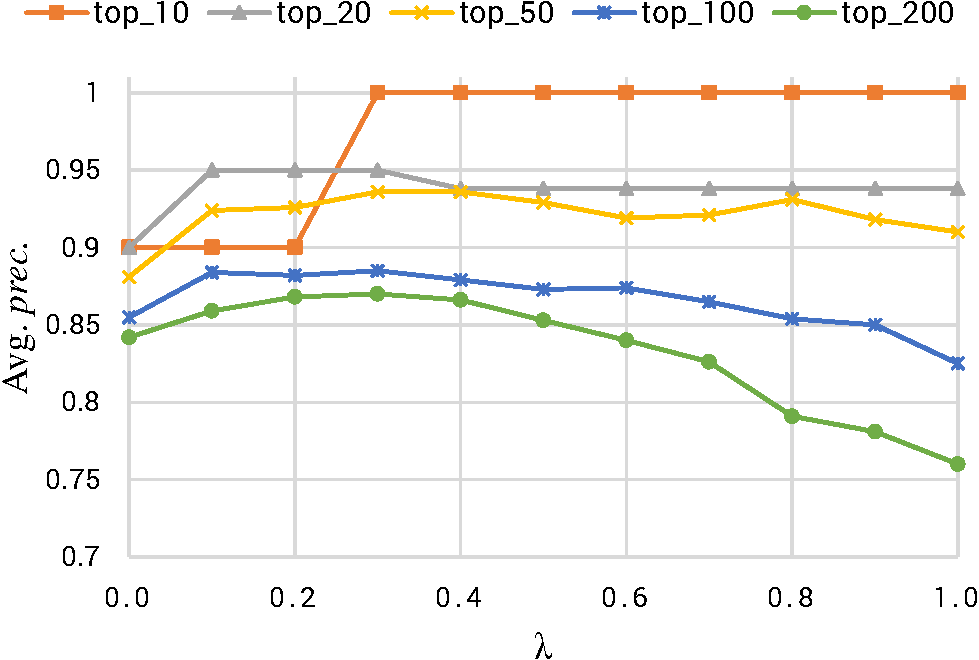
\includegraphics[width=0.5\textwidth]{figures/fb15k_hole_conf-crop.pdf} }}
%    \subfloat[Confidence + SSP]{{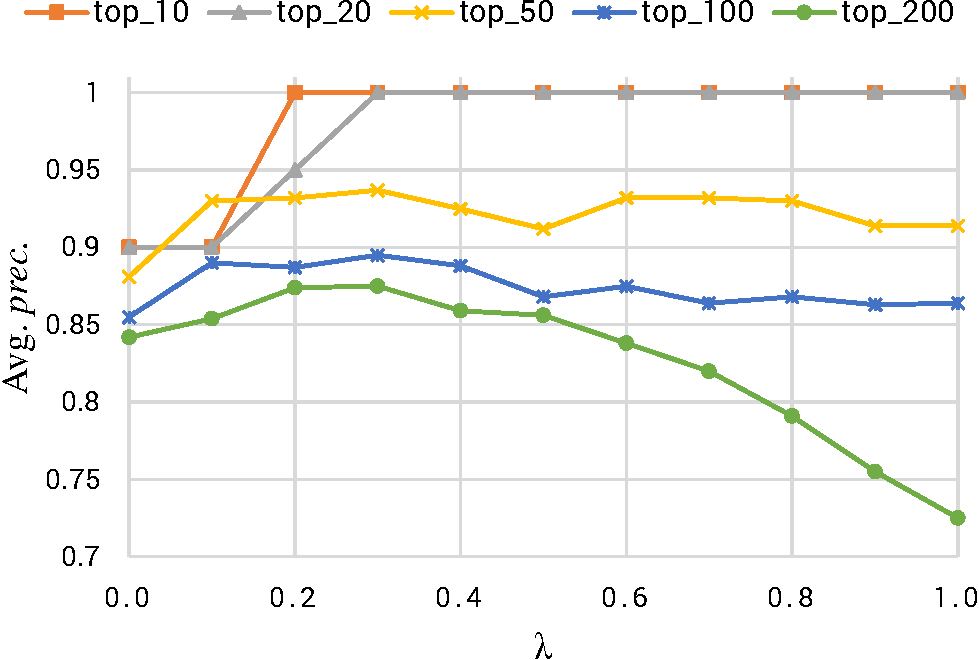
\includegraphics[width=0.5\textwidth]{figures/fb15k_ssp_conf-crop.pdf} }}\\
%    \subfloat[PCA Confidence + HolE]{{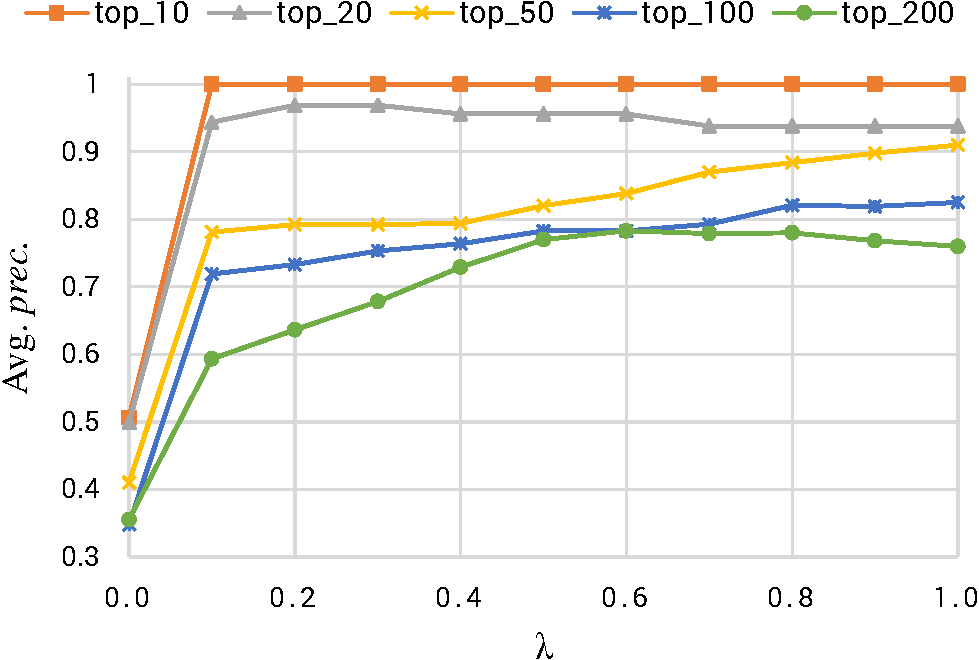
\includegraphics[width=0.5\textwidth]{figures/fb15k_hole_pca-crop.pdf} }}
%    \subfloat[PCA Confidence + SSP]{{\includegraphics[width=0.5\textwidth]{figures/fb15k_ssp_pca-crop.pdf} }}    
%    \caption{Average prediction score of some top rules on FB15K dataset with the hybrid rule quality scoring function.}
%    \label{fig:fb15k}
%\end{figure}
%
%\begin{figure}[t]
%    \centering
%    \subfloat[Confidence + TransE]{{\includegraphics[width=0.5\textwidth]{figures/wiki44k_transe_conf-crop.pdf} }}
%    \subfloat[Confidence + SSP]{{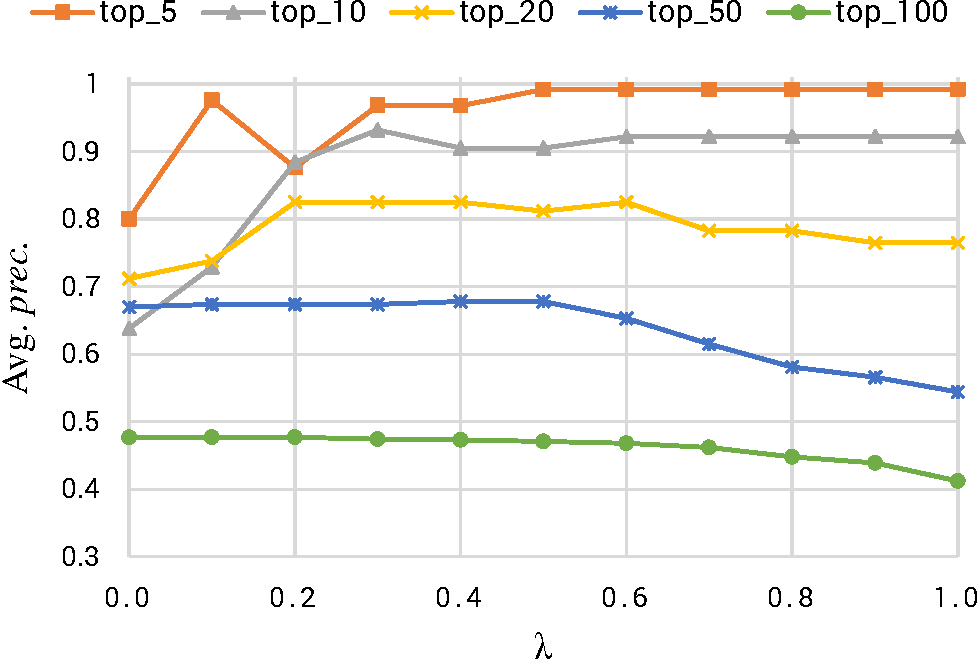
\includegraphics[width=0.5\textwidth]{figures/wiki44k_ssp_conf-crop.pdf} }}\\
%    \subfloat[PCA Confidence + TransE]{{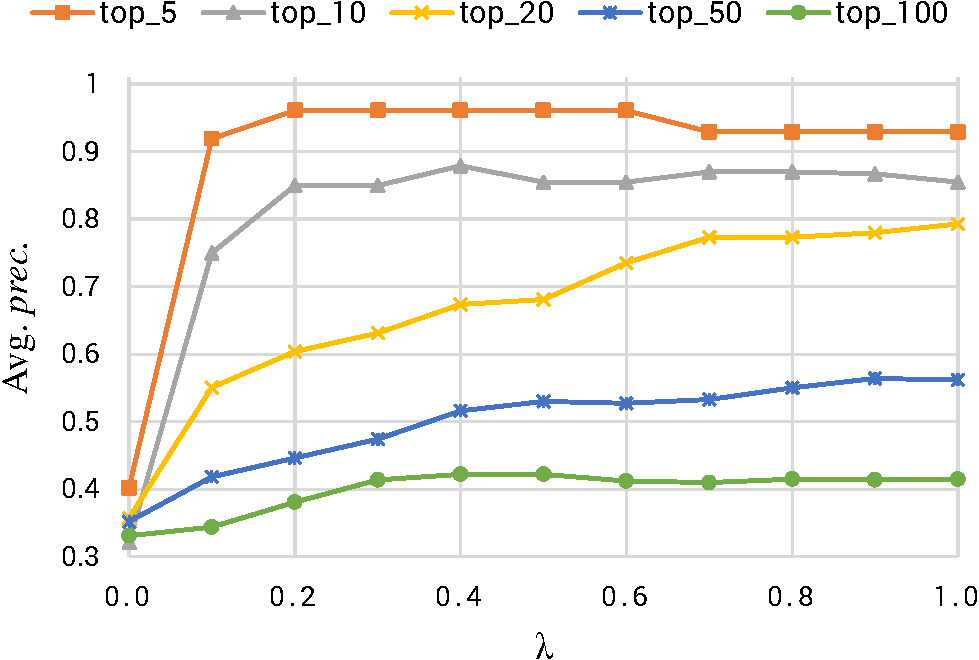
\includegraphics[width=0.5\textwidth]{figures/wiki44k_transe_pca-crop.pdf} }}
%    \subfloat[PCA Confidence + SSP]{{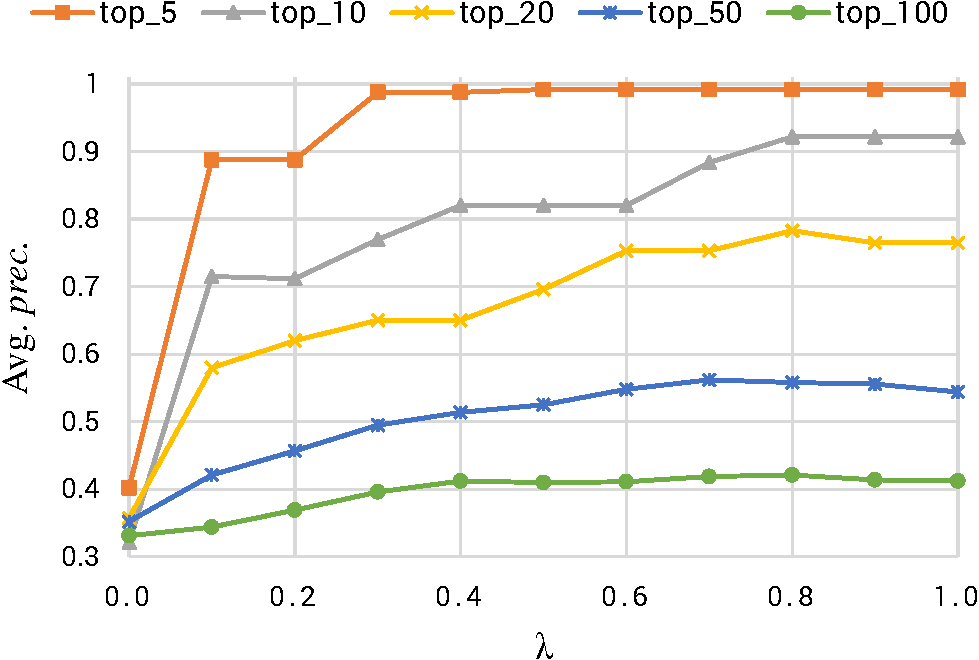
\includegraphics[width=0.5\textwidth]{figures/wiki44k_ssp_pca-crop.pdf} }}    
%    \caption{Average prediction score of some top rules on WIKI44K dataset with the hybrid rule quality scoring function.}
%    \label{fig:wiki44k}
%\end{figure}



%The higher the prediction score is, the better the rule is. Figures \ref{fig:fb15k} and \ref{fig:wiki44k} demonstrate the average prediction score of top $k$ rules on FB15K and WIKI44K datasets when using hybrid quality with different traditional rule-based measures and values of embedding weights $\lambda$. We can see that with each top $k$ rules, their average prediction score rises along with the increasing of parameter $\lambda$ until reaching some optimal value, then falls down until $\lambda$ is equal to 1. Hence, the combination of $q_{rm} $ and $q_{es}$ is crucial to achieve the best result. In addition, the hybrid quality works better than the traditional PCA confidence with every value of $\lambda$. The reason is that our training KG $\cG^a$ is randomly sampled that break the assumption made by PCA confidence. 











